\documentclass[11pt]{article}
\usepackage[utf8]{inputenc}
\usepackage[russian]{babel}
\usepackage[T1]{fontenc}
\usepackage{amssymb,amsmath,clrscode,graphicx,indentfirst}

\author{Иван Веселов}
\title{Курс kiev-clrs -- Лекция 1. Анализ алгоритмов}
\date{10 января 2009 г.}

\begin{document}

\maketitle
\tableofcontents
\newpage

\setlength{\parskip}{1ex plus 0.5ex minus 0.2ex}

\section{Цель лекции}
\begin{itemize}
\item Изучить средства описания и анализа алгоритмов
\item Рассмотреть сортировку слиянием и сортировку вставкой
\item Начать использовать асимптотическую нотацию для выражения времени
  выполнения алгоритмов
\item Рассмотреть технику ``разделяй и властвуй'' в контексте сортировки
  слиянием
\end{itemize}

\section{Введение}
В рамках данного курса изучаются два аспекта:
\begin{itemize}
  \item анализ алгоритмов
  \item дизайн алгоритмов
\end{itemize}

Мы начнём с анализа, т.к. перед тем, как что-то проектировать и создавать, нужно
узнать критерии, определяющие насколько хорошо то, что у нас получается. Эти
критерии и изучает анализ алгоритмов. Таким образом, анализ алгоритма -- это
теоретическое изучение производительности программ и использования ими ресурсов.

Но давайте будем реалистами и подумаем над тем, что есть вещи, которые могут
быть важнее производительности в контексте разработки программ (спросить какие):

\begin{itemize}
\item корректность
\item простота
\item надёжность
\item затраты на разработку (время, затраченное программистом)
\item лёгкость в поддержке
\item масштабируемость
\item модульность
\item безопасность
\end{itemize}

Может тогда изучение алгоритмов нам и не нужно? Нужно, так как:

\begin{itemize}
\item они помогают понять масштабируемость
\item проводят границу между пригодностью и непригодностью кода,
т.е. медленный алгоритм зачастую просто неприменимы для больших входных данных.
\item они определяют язык, в терминах которого можно говорить о поведении программ
\item скорость - это круто!

   Производительность - как деньги, которыми можно расплачиваться за всё
   остальное, если у вас есть производительность -- можно обменять часть её
   на дополнительные ``фичи'', другую часть -- на масштабируемость и т.д.

\item развивают логическое мышление
\end{itemize}

\section{Сортировка вставкой}
Задача сортировки:

\emph{Вход}: последовательность чисел $\langle a_1, a_2, \ldots, a_n \rangle$

\emph{Выход}: перестановка $\langle a_1', a_2', \ldots, a_n' \rangle$ такая, что
$a_1' \leqslant a_2' \leqslant ... \leqslant a_n'$ (монотонно возрастающая)

Для описания алгоритмов важно использовать чёткий и выразительный язык. Часто,
хорошим вариантом является естественный язык -- например русский или английский.
Однако, когда необходимо более чёткое и точное понимание всего происходящего в
программе мы будем использовать \emph{псевдокод}.

Алгоритм сортировки вставкой: 
\nopagebreak
\begin{codebox}
\Procname{$\proc{Insertion-Sort}(A, n)$ \Comment sorts $A[1 \twodots n]$}
\li \For $j \gets 2 $ \To $n$
\li     \Do $key \gets A[j]$
\li         $i \gets j - 1$
\li         \While $i > 0$ and $A[i] > key$
\li             \Do $A[i+1] \gets A[i]$
\li                 $i \gets i - 1$
               \End
\li         $A[i+1] \gets key$
        \End
\End
\end{codebox}

\begin{figure}[ht]
  \centering
  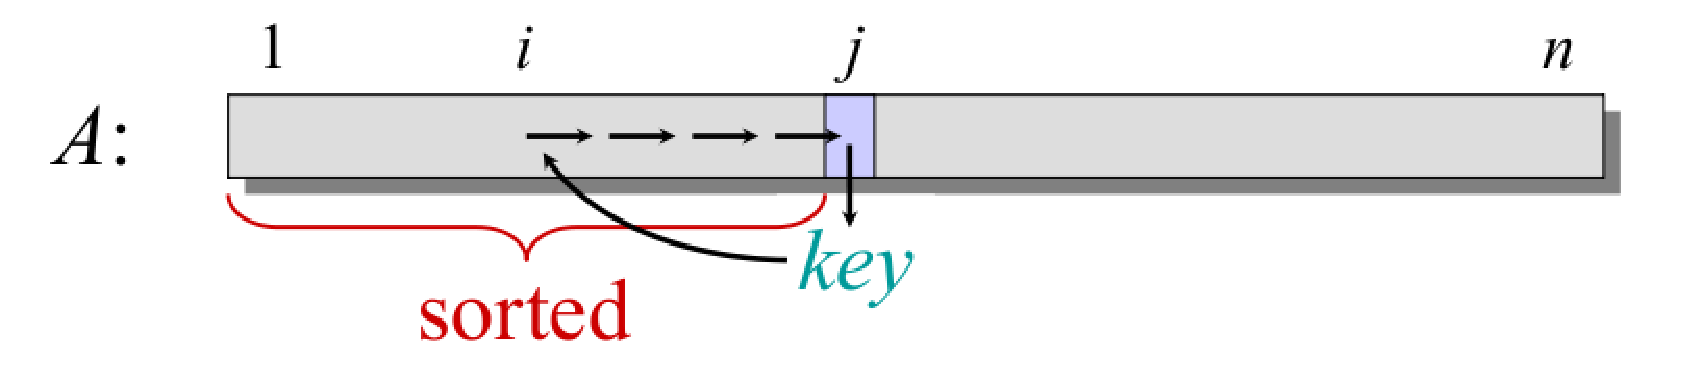
\includegraphics[width=3in]{lecture1/insert.eps}
  \caption{Принцип сортировки вставкой}
  \label{fig:insert}
\end{figure}

То, что часть начало массива является постоянно отсортированным -- является
\emph{инвариантом цикла}, то есть таким свойством, которое не меняется при
выполнении цикла. С помощью инвариантов доказывается \emph{корректность}
алгоритма. Это напоминает метод математической индукции: сначала доказывается,
что инвариант выполняется до начала цикла (базис индукции), затем, предположив,
что свойство выполняется при счётчике цикла равном $N - 1$ (гипотеза индукции)
доказывается, что он останется верным и при $N$. Это можно сравнить с подъёмом
по ступенькам: если мы знаем, что можем подняться на первую ступеньку и знаем,
что можем переступить на следующую -- то это означает, что можно подняться до
самого конца лестницы. И наконец последний шаг доказательства корректности
алгоритма -- это убедиться, что при завершении главного цикла мы получаем
решение поставленной задачи (этого шага нет в математической индукции).

\begin{figure}[ht]
  \centering
  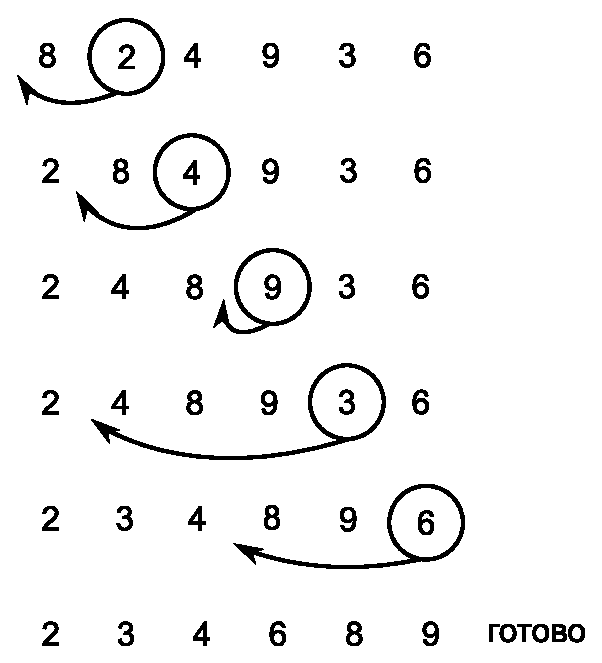
\includegraphics[width=3in]{lecture1/insert-sort-example.eps}
  \caption{Пример сортировки вставкой}
  \label{fig:insertion-sort-example}
\end{figure}

Время работы алгоритма:
\begin{itemize}
\item зависит от входных данных (например они могут быть уже отсортированными)
\item зависит от размера входных данных
\end{itemize}

Таким образом, можно параметризовать время работы по размеру входных данных
алгоритма. При этом мы хотим получить верхнюю границу оценки (наихудшее время),
чтобы обеспечить некие гарантии пользователю алгоритма.

\section{Виды анализа}
Можно рассматривать разные случаи:

\begin{itemize}
\item анализ наихудшего случая (worst-case analysis) -- обычно мы будем
  проводить именно его.

  $T(n) = $ максимальному времени для любых входных данных размера $n$

\item анализ среднего случая (average case) -- иногда будем проводить и его.

  $T(n) = $ ожидаемому в среднем времени для всех вариантов входных данных
  размера $n$.

  Здесь нам нужны знания или предположения о том, что именно представляют собой
  данные, то есть как они статистически распределены. Часто можно предположить
  что все входные данные -- равновероятны.

\item анализ наилучшего случая (best case) -- от него мало толку, т.к. можно
  придумать алгоритм, который будет хорошо работать для каких-то конкретных
  данных и очень плохо для всех остальных, проанализировать лучший случай и
  радоваться какой классный у нас алгоритм.
\end{itemize}

Вернёмся к сортировке вставкой. Какое время работы в наихудшем случае для этого
алгоритма?

Это зависит от конкретного компьютера:
\begin{itemize}
\item относительная скорость -- на одной и той же машине
\item абсолютная скорость -- на разных машинах
\end{itemize}

Здесь нас озаряет \emph{великая идея}!
\begin{itemize}
\item игнорировать машинно-зависимые константы
\item рассматривать не само время, а его рост, то есть на поведение функции
  $T(n)$, когда $n \rightarrow \infty$
\end{itemize}

\section{$\Theta$-нотация}
Асимптотическая оценка функции.

Математически определяется как:
\begin{equation*}
  \Theta(g(n)) = \{ f(n): \exists c_1, c_2 > 0 \text{ и } n_0
  \text{ такие, что }
  0 \leqslant c_1 g(n) \leqslant f(n) \leqslant c_2 g(n), \forall n > n_0
  \}
\end{equation*}

Разбирать это мы пока не будем, и в данный момент мы будем определять оценку
функции с помощью таких действий:
\begin{itemize}
\item отбросить от функции члены младшего порядка
\item игнорировать множители-константы
\end{itemize}

Примеры:
\begin{equation*}
5n^3 + 2n^2 - 10n + 657 = \Theta(n^3)
\end{equation*}
\begin{equation*}
-7n^2 + 2n + 2 = \Theta(n^2)
\end{equation*}

\begin{figure}[ht]
  \centering
  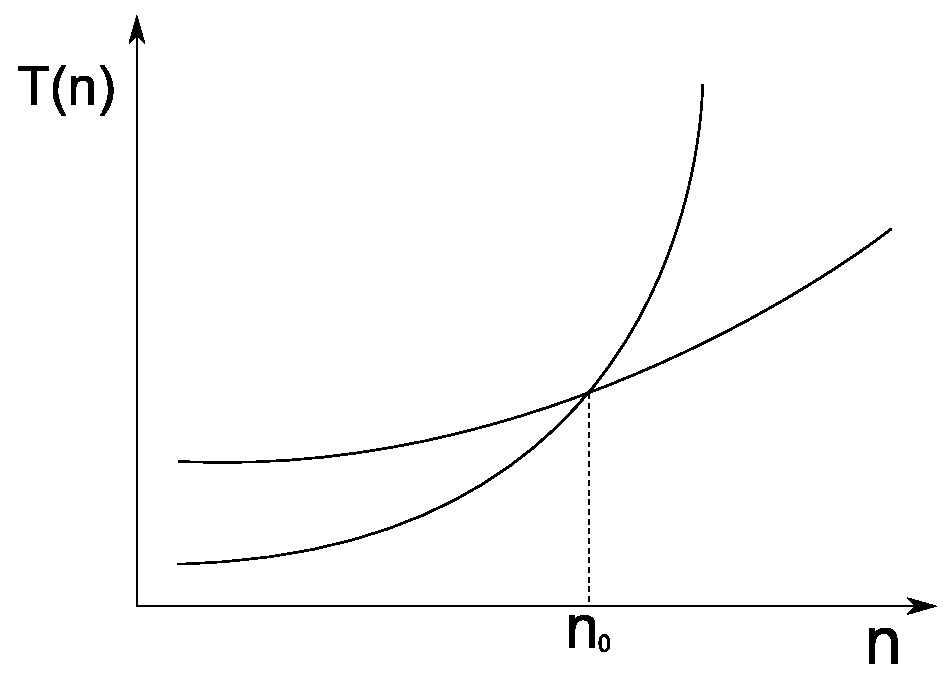
\includegraphics[width=3in]{lecture1/theta-beats.eps}
  \caption{Сравнение двух полиномиальных оценок}
  \label{fig:thetas-comparison}
\end{figure}

Поскольку нас интересует поведение функций, когда $n \rightarrow \infty$, то
становится понятно, что алгоритм $\Theta(n^2)$ рано или поздно ``победит'' алгоритм
$\Theta(n^3)$

\section{Анализ сортировки вставкой}

Худший случай входных данных для этого алгоритма -- это массив отсортированный в
обратном порядке (при этом получается больше всего перестановок).

\begin{equation*}
  T(n) = \sum_{j-2}^n{\Theta(j)} = \Theta(n^2) \text{ (арифметическая прогрессия)}
\end{equation*}

Быстр ли алгоритм сортировки вставкой? 
\begin{itemize}
\item для маленьких $N$ -- его скорость вполне приемлема
\item для больших $N$ -- нет (квадратичная скорость сортировки -- это медленно)
\end{itemize}

\section{Сортировка слиянием}

Существуют несколько разных подходов к созданию алгоритмов, например тот, что
был рассмотрен в сортировке вставкой -- называется \textbf{инкрементным}: каждый
раз у нас был уже отсортированный массив меньшего размера и мы постепенно
добавляли к нему по одному новому элементу в нужное место.

Теперь мы кратко рассмотрим другой подход, который называется методом
\textbf{декомпозиции} или \textbf{разделения} (``разделяй и властвуй''). Многие
алгоритмы имею рекурсивную структуру, то есть вызывают себя один или несколько
раз для выполнения некоторой полезной подзадачи. Обычно такие алгоритмы как раз
и разрабатываются методом декомпозиции.

Суть метода декомпозиции -- три этапа:
\begin{itemize}
\item \emph{Разделение} -- разбиение задачи на подзадачи меньшего размера
\item \emph{Покорение} -- решение этих задач рекурсивным образом
\item \emph{Объединение} -- получение решения основной задачи из решений меньших
\end{itemize}

Алгоритмом именно такого типа является сортировка слиянием (merge sort). Схема
работы процедуры Merge-sort($A[1 \twodots n]$) (оставить место слева для
$\Theta$-оценок):

\begin{enumerate}
\item Если $n = 1$ -- готово, выдать $A$
\item Рекурсивно отсортировать массивы $A[1 \twodots \lceil n/2 \rceil]$ и $A[\lfloor
  n/2 \rfloor+1 \twodots n]$
\item Объединить их (merge)
\end{enumerate}

Таким образом основная процедура, в которой выполняется работа -- объединение.
Рассмотрим как можно объединить два уже отсортированных массива:

\begin{figure}[ht]
  \centering
  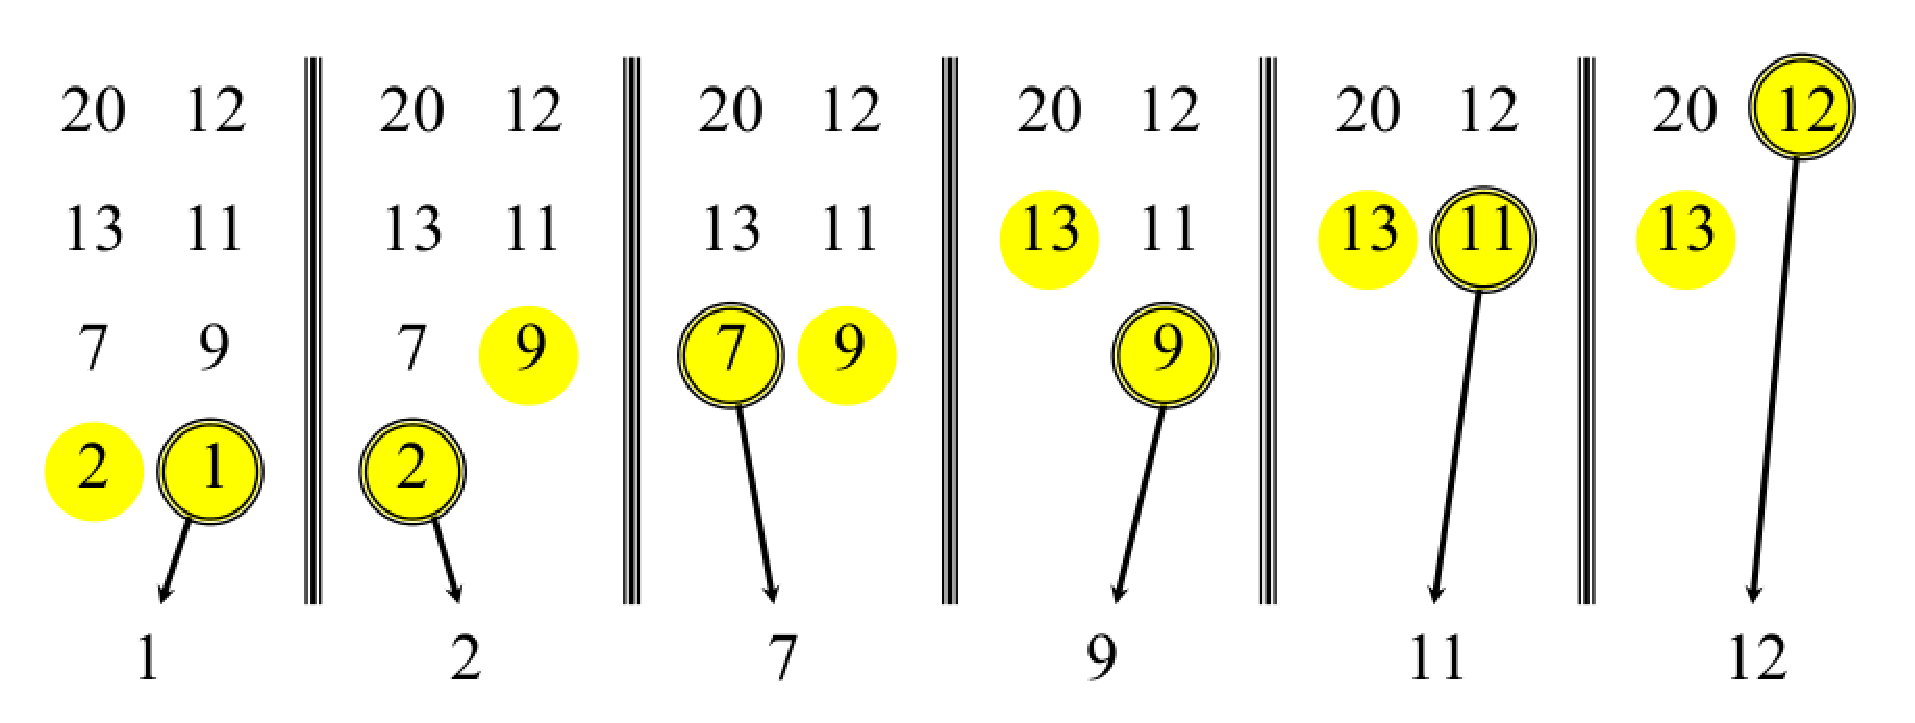
\includegraphics[width=4in]{lecture1/merge.eps}
  \caption{Процедура слияния}
  \label{fig:merge}
\end{figure}

(Можно описать как пример с двумя стопками отсортированных карт).

Поскольку нужно сделать как максимум $n$ сравнений и каждое сравнение можно
считать атомарной операцией ($\Theta(1)$) -- получаем $\Theta(n)$.

Теперь запишем все шаги алгоритма и их оценки:

\begin{tabular}{|r|l|}
$\Theta(1)$    & 1. Если $n = 1$ -- готово  \\
$2\Theta(n/2)$ & 2. Отсортировать $A[1 \twodots \lceil n/2 \rceil]$ и $A[\lfloor
                    n/2 \rfloor+1 \twodots n]$ \\
$\Theta(n)$    & 3. Объединить их (merge) 
\end{tabular}

Во втором пункте допущена некоторая неточность -- мы приблизили всё к $n/2$,
однако можно показать, что апроксиматически это ни на что не влияет.

Таким образом, получаем рекуррентное соотношение:
\begin{equation}
  T(n) = \begin{cases}
    \Theta(1), \text{ если } n = 1 \\
    2\Theta(n/2) + \Theta(n), \text{ если } n > 1
    \end{cases}
  \label{eq:recur}
\end{equation}

Обычно мы можем пренебречь случаем, когда $T(n) = \Theta(1)$ для достаточно
малых $n$, т.к. он не играет роли при асимптотической оценке, но следует быть
внимательными.

В следующей лекции мы изучим несколько методов для получения решений подобных
рекуррентностей, а сейчас мы только кратко продемонстрируем один из методов.

\section{Дерево рекурсии}
Преобразовываем нашу задачу к виду: $T(n) = 2T(n/2) + cn$, где константа $c > 0$.
И начинаем выписывать сумму в виде дерева:

\begin{figure}[ht]
  \centering
  
\includegraphics[width=0.5in]{lecture1/tree1.eps}
  \caption{Дерево рекурсии -- корневой узел}
  \label{fig:rectree1}
\end{figure}

Разворачиваем согласно соотношению \ref{eq:recur} (см. рис. \ref{fig:rectree2}, \ref{fig:rectree3})

\begin{figure}[ht]
  \centering
  
\includegraphics[width=2in]{lecture1/tree2.eps}
  \caption{Дерево рекурсии -- шаг второй}
  \label{fig:rectree2}
\end{figure}

\begin{figure}[ht]
  \centering
  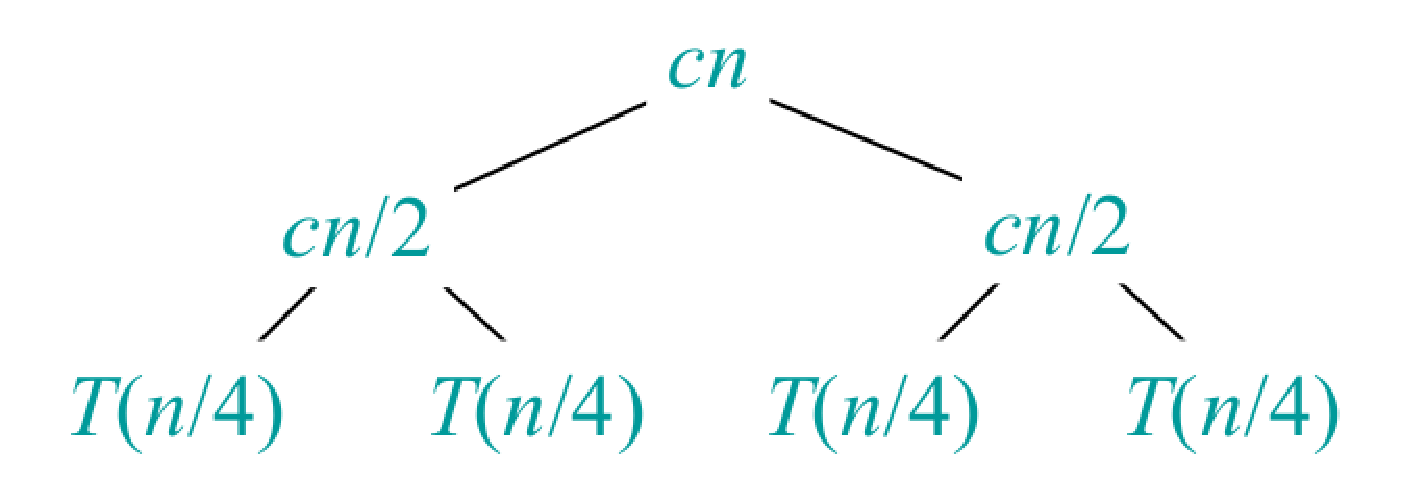
\includegraphics[width=3in]{lecture1/tree3.eps}
  \caption{Дерево рекурсии -- шаг третий}
  \label{fig:rectree3}
\end{figure}

Самые нижние узлы дерева (листья) -- это подзадачи размером 1, то есть уже
массивы длины 1, которые естественно отсортированы, потому никакой работы по их
сортировке проводить не надо, потому в листьях пишется $\Theta(1)$ (см. рис.
\ref{fig:rectree4})

\begin{figure}[ht]
  \centering
  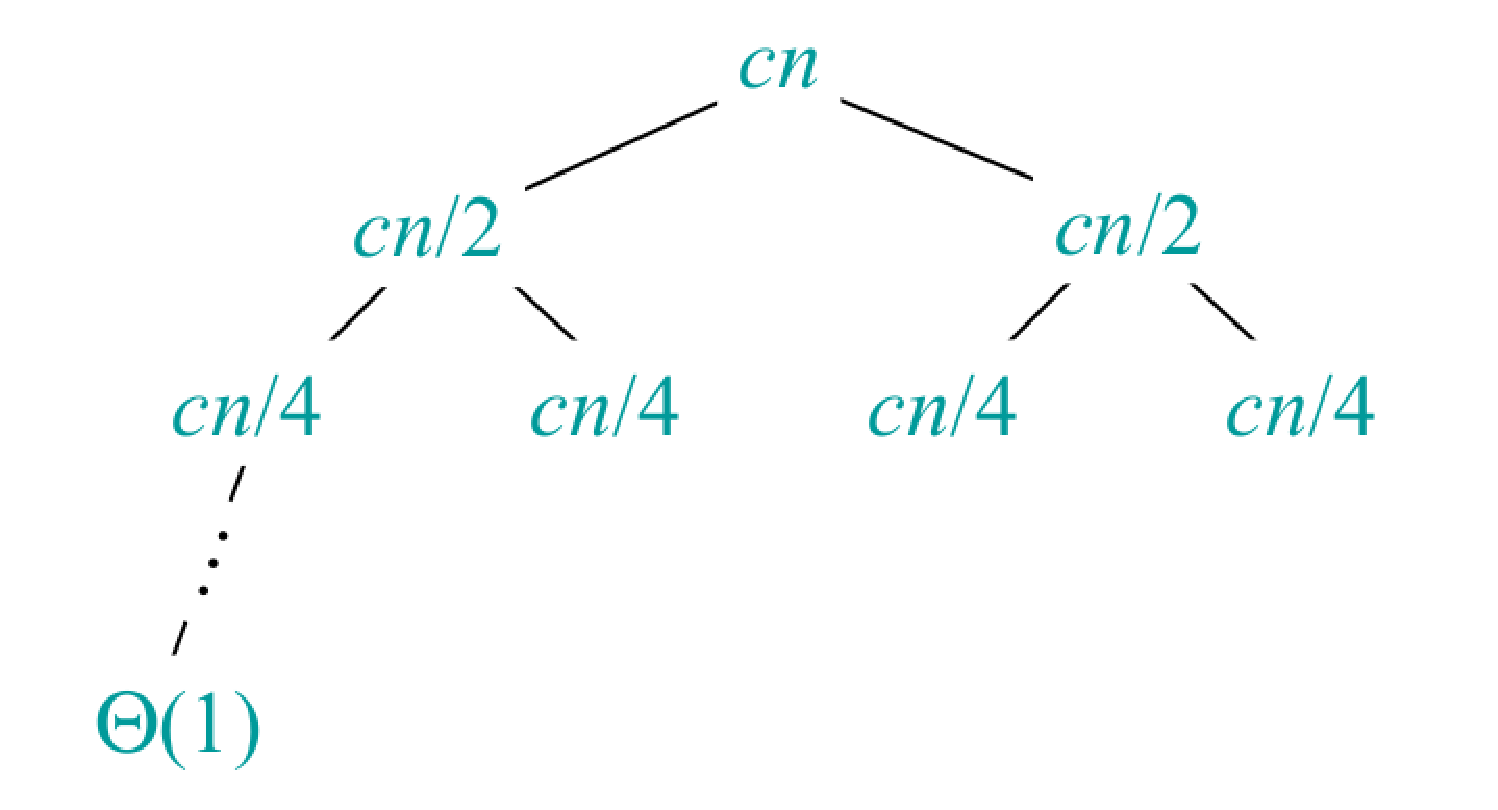
\includegraphics[width=3.5in]{lecture1/tree4.eps}
  \caption{Дерево рекурсии с листьями $\Theta(1)$}
  \label{fig:rectree4}
\end{figure}

Поскольку каждые раз происходит уменьшение задачи вдвое, то определение высоты
дерева по сути является эквивалентным вопросу -- ``сколько раз нужно поделить
число на два, чтобы получить 1'', и ответ на него -- $lg n$, то есть двоичный
логарифм (мы будем использовать обозначения из книги, несмотря на то, что в
русскоязычной литературе принято обозначать так десятичный логарифм). Рис.
\ref{fig:rectree5}

\begin{figure}[ht]
  \centering
  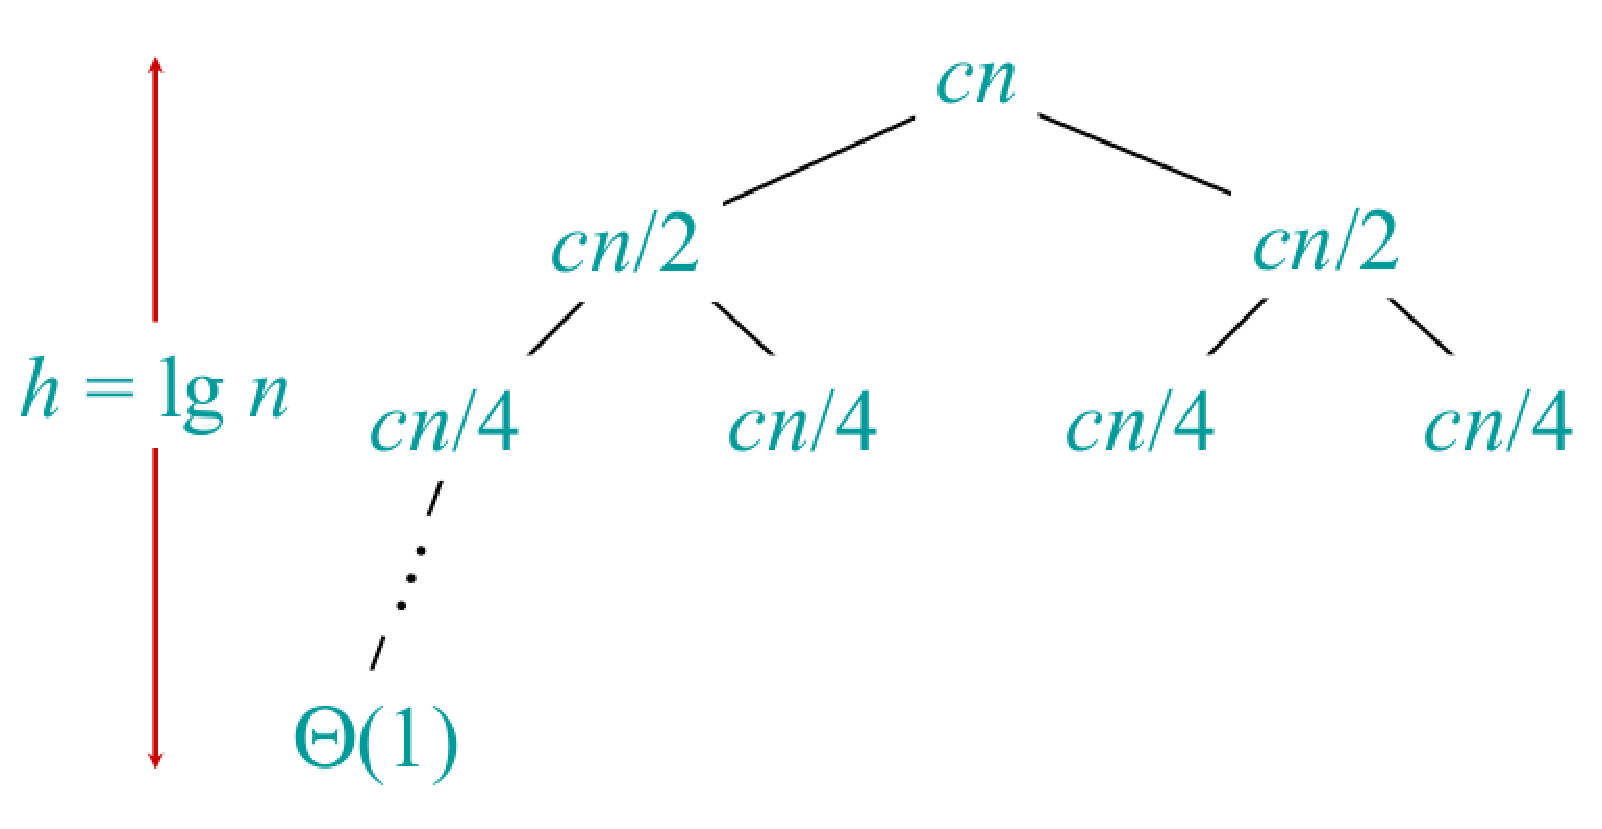
\includegraphics[width=4in]{lecture1/tree5.eps}
  \caption{Дерево рекурсии с указанной высотой}
  \label{fig:rectree5}
\end{figure}

Теперь начнём суммировать значения в узлах дерева по уровням. 
(см. рис. \ref{fig:rectree6}, \ref{fig:rectree7}, \ref{fig:rectree8})

\begin{figure}[ht]
  \centering
  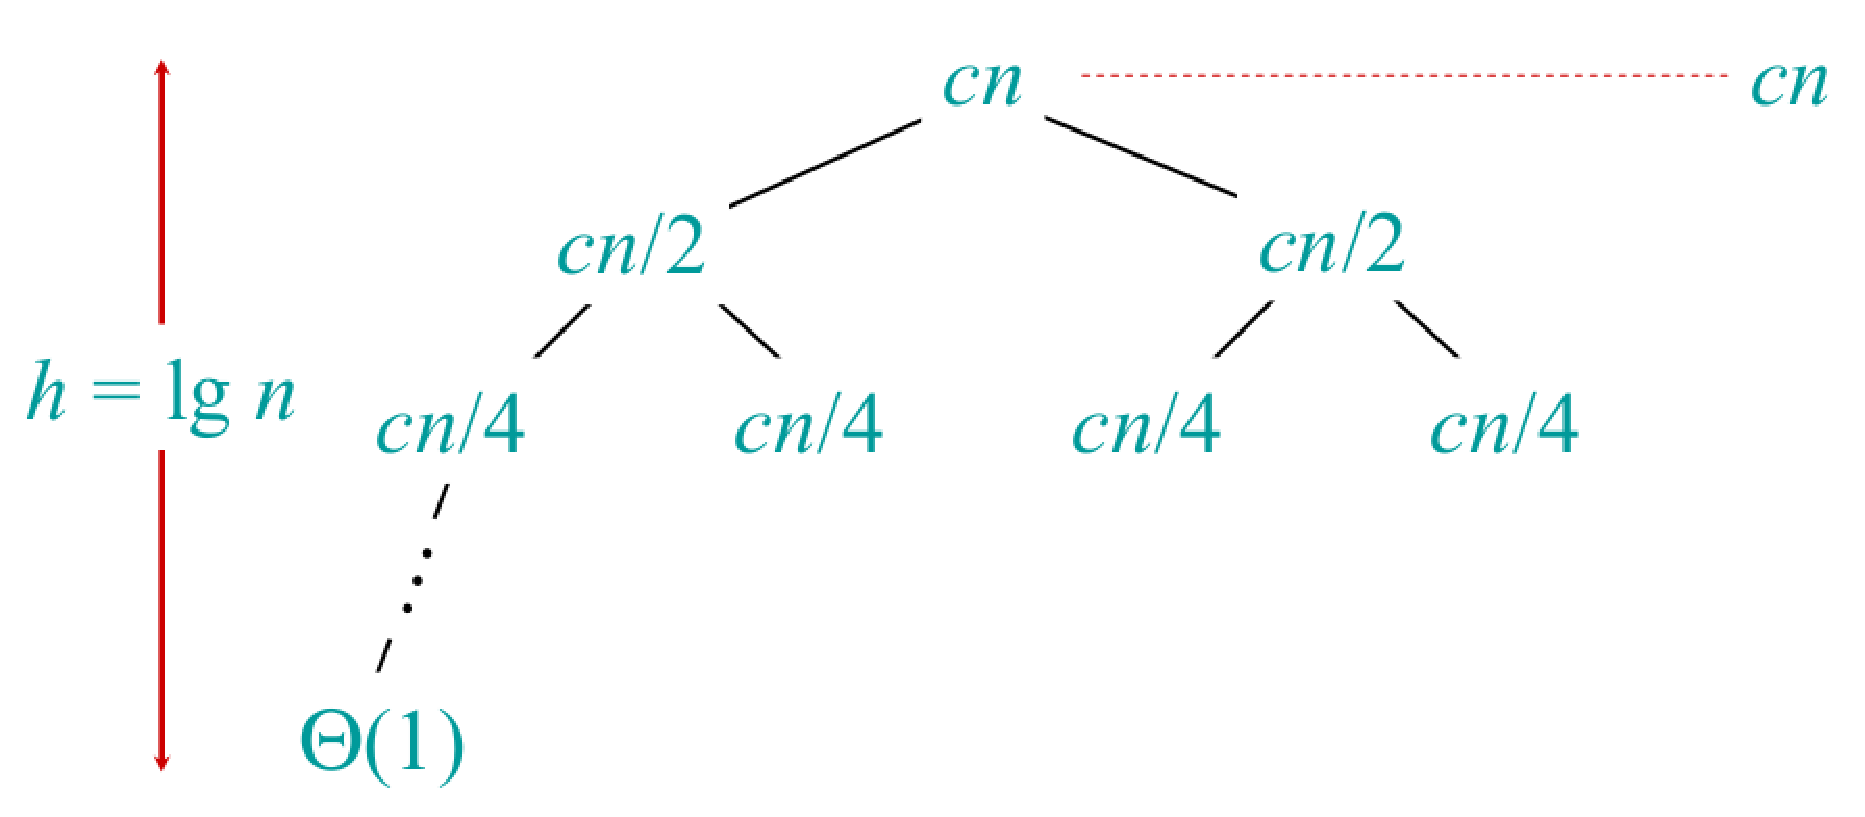
\includegraphics[width=4in]{lecture1/tree6.eps}
  \caption{Дерево рекурсии с суммой уровня 1}
  \label{fig:rectree6}
\end{figure}

\begin{figure}[ht]
  \centering
  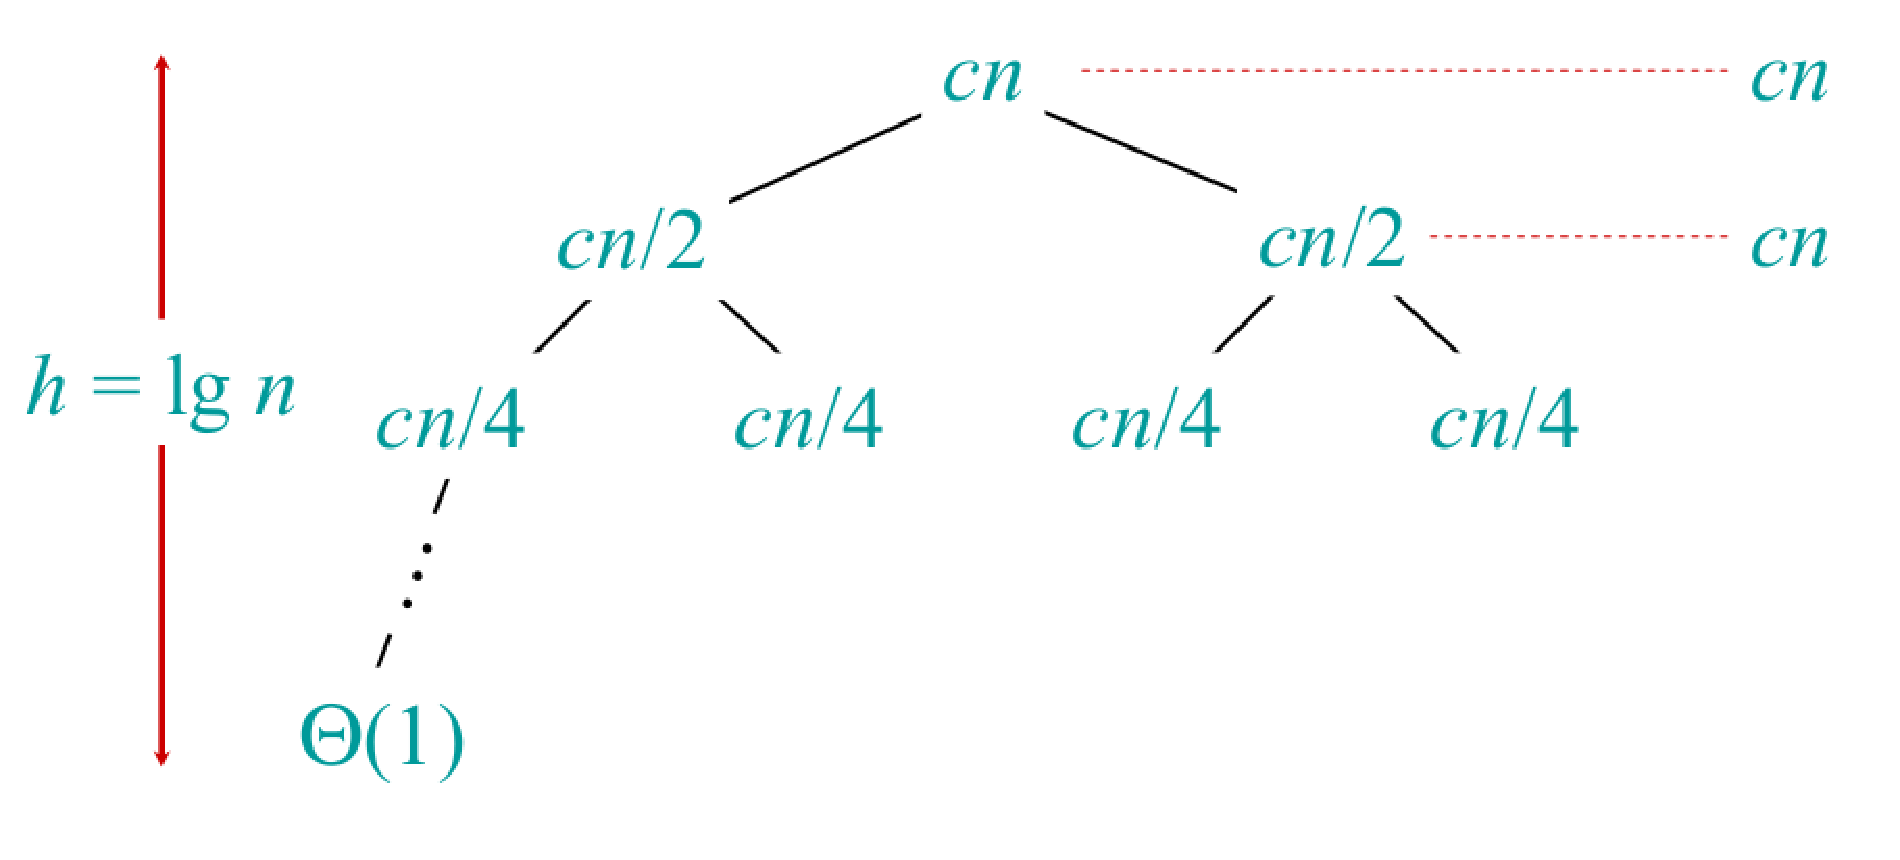
\includegraphics[width=4in]{lecture1/tree7.eps}
  \caption{Дерево рекурсии с суммой уровней 1-2}
  \label{fig:rectree7}
\end{figure}

\begin{figure}[ht]
  \centering
  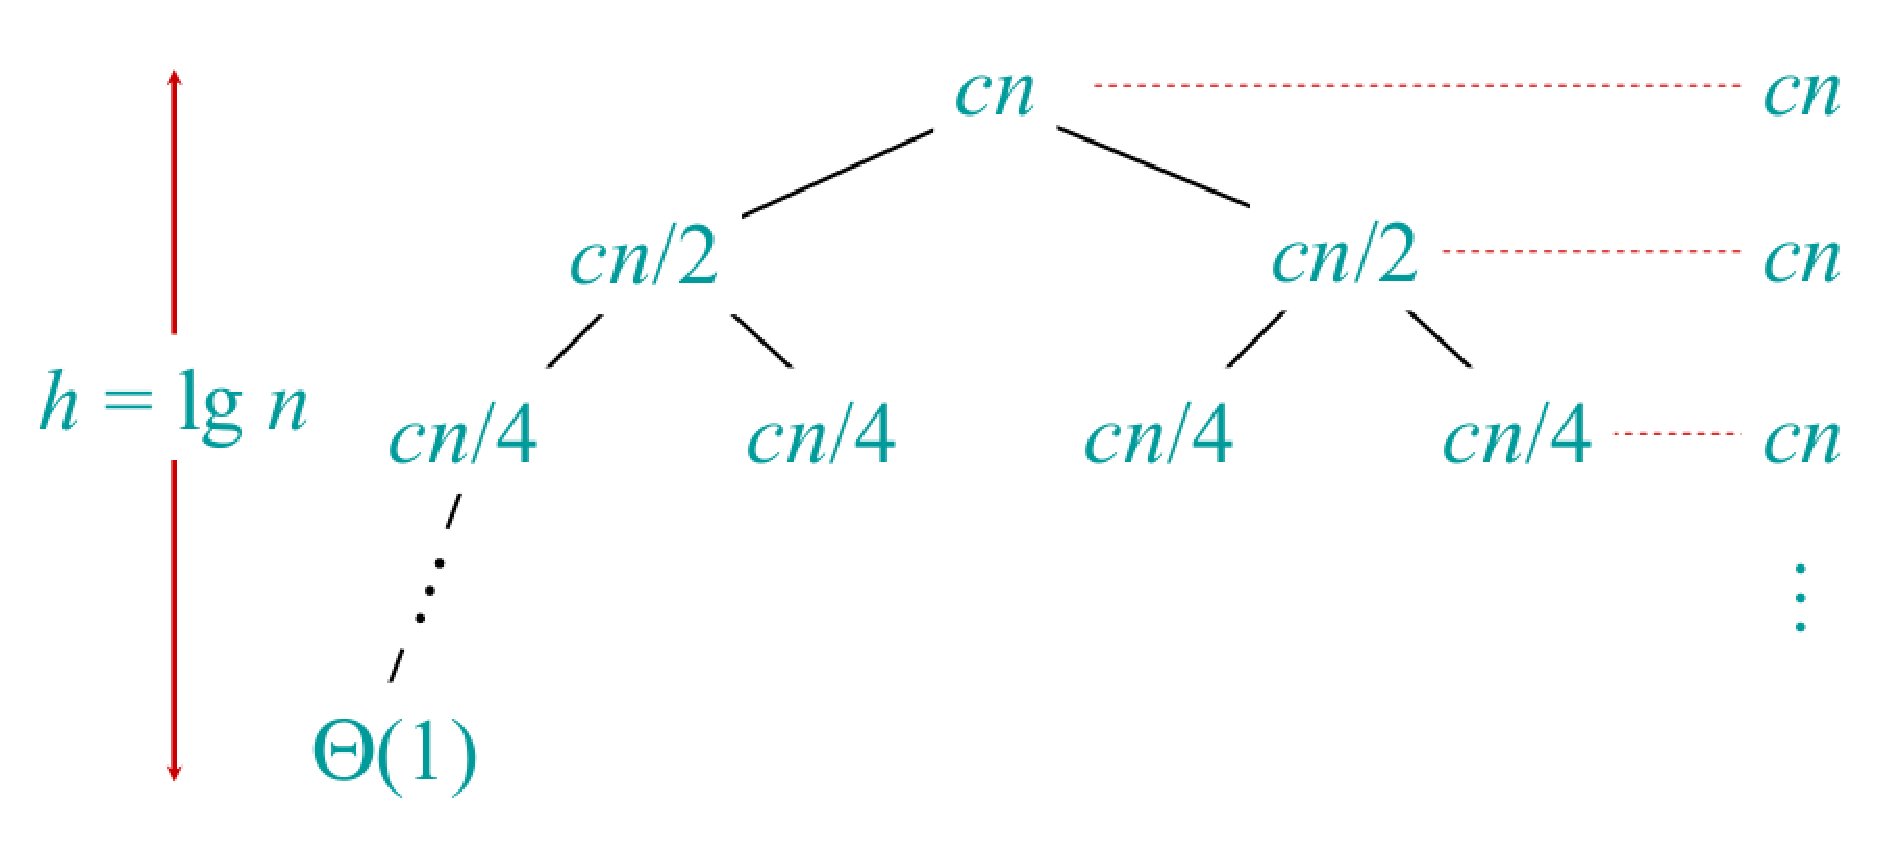
\includegraphics[width=4in]{lecture1/tree8.eps}
  \caption{Дерево рекурсии с суммой уровней 1-3}
  \label{fig:rectree8}
\end{figure}

Наконец просуммируем уровень листьев -- самых нижних узлов дерева, т.к. их $n$,
умножая на $\Theta(1)$ получим $\Theta(n)$ (см. рис. \ref{fig:rectree9})

\begin{figure}[ht]
  \centering
  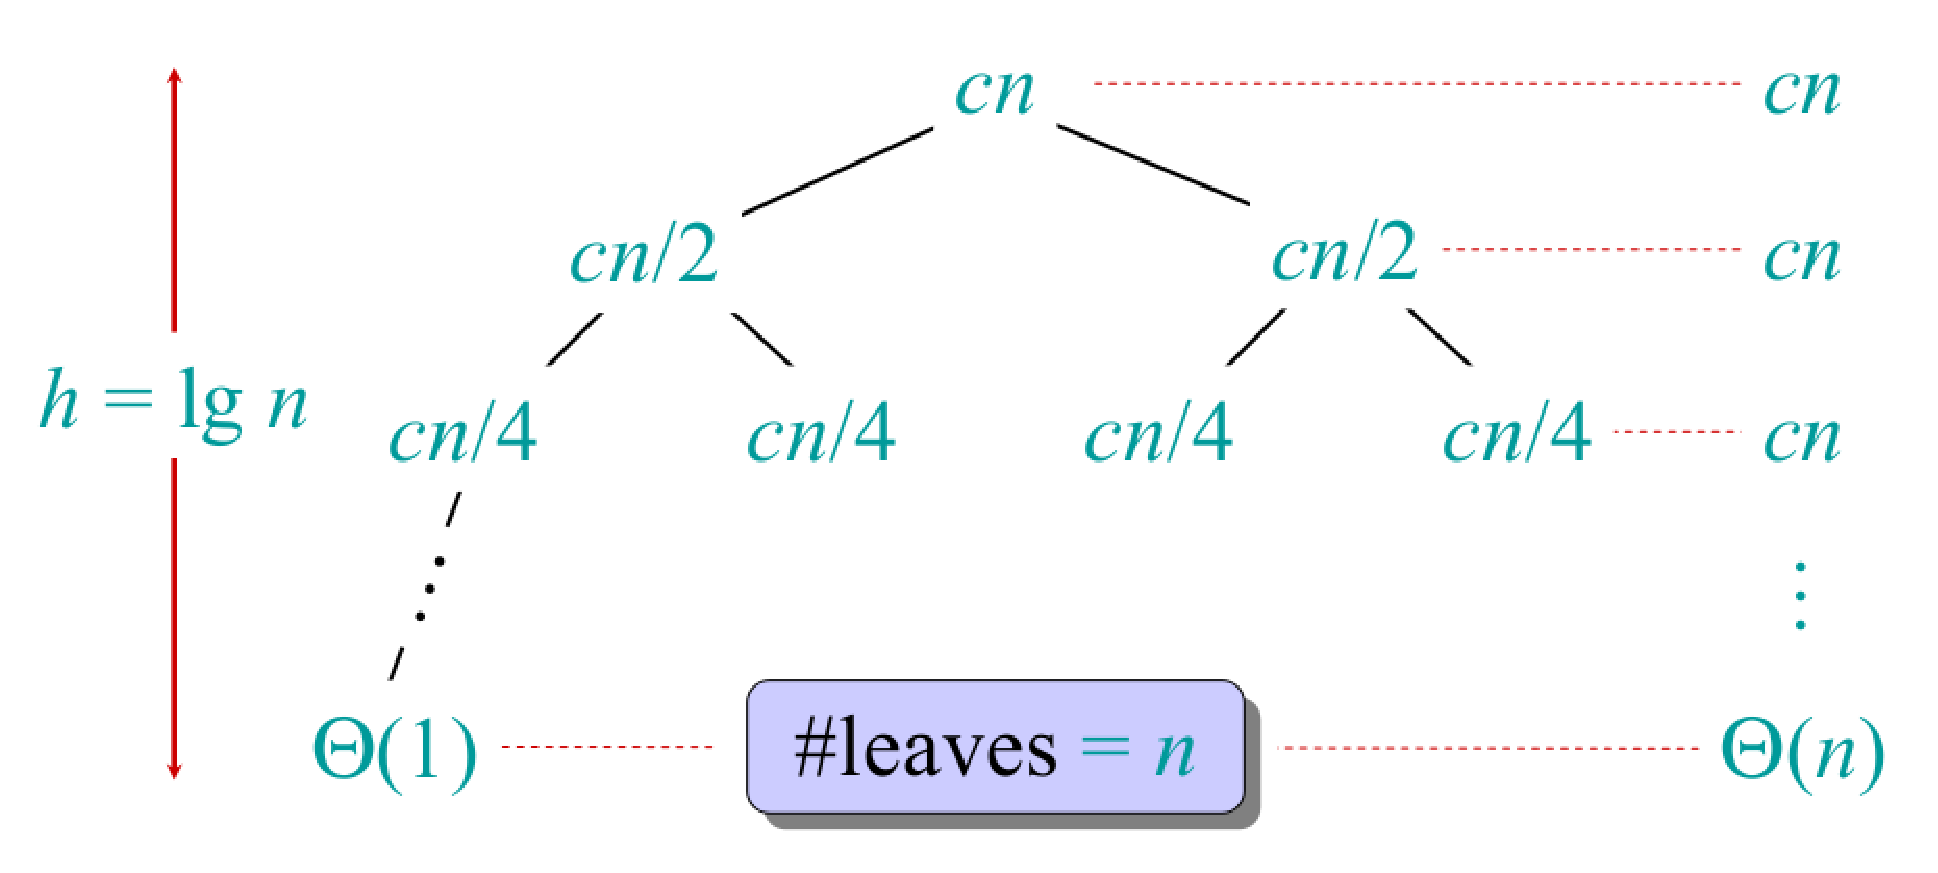
\includegraphics[width=4in]{lecture1/tree9.eps}
  \caption{Дерево рекурсии с суммой значений в листьях}
  \label{fig:rectree9}
\end{figure}

Теперь просуммируем значения сумм всех уровней, чтобы определить оценку для
всего алгоритма, в итоге получаем $\Theta(n lg n)$ (см. рис.
\ref{fig:rectree10})

\begin{figure}[ht]
  \centering
  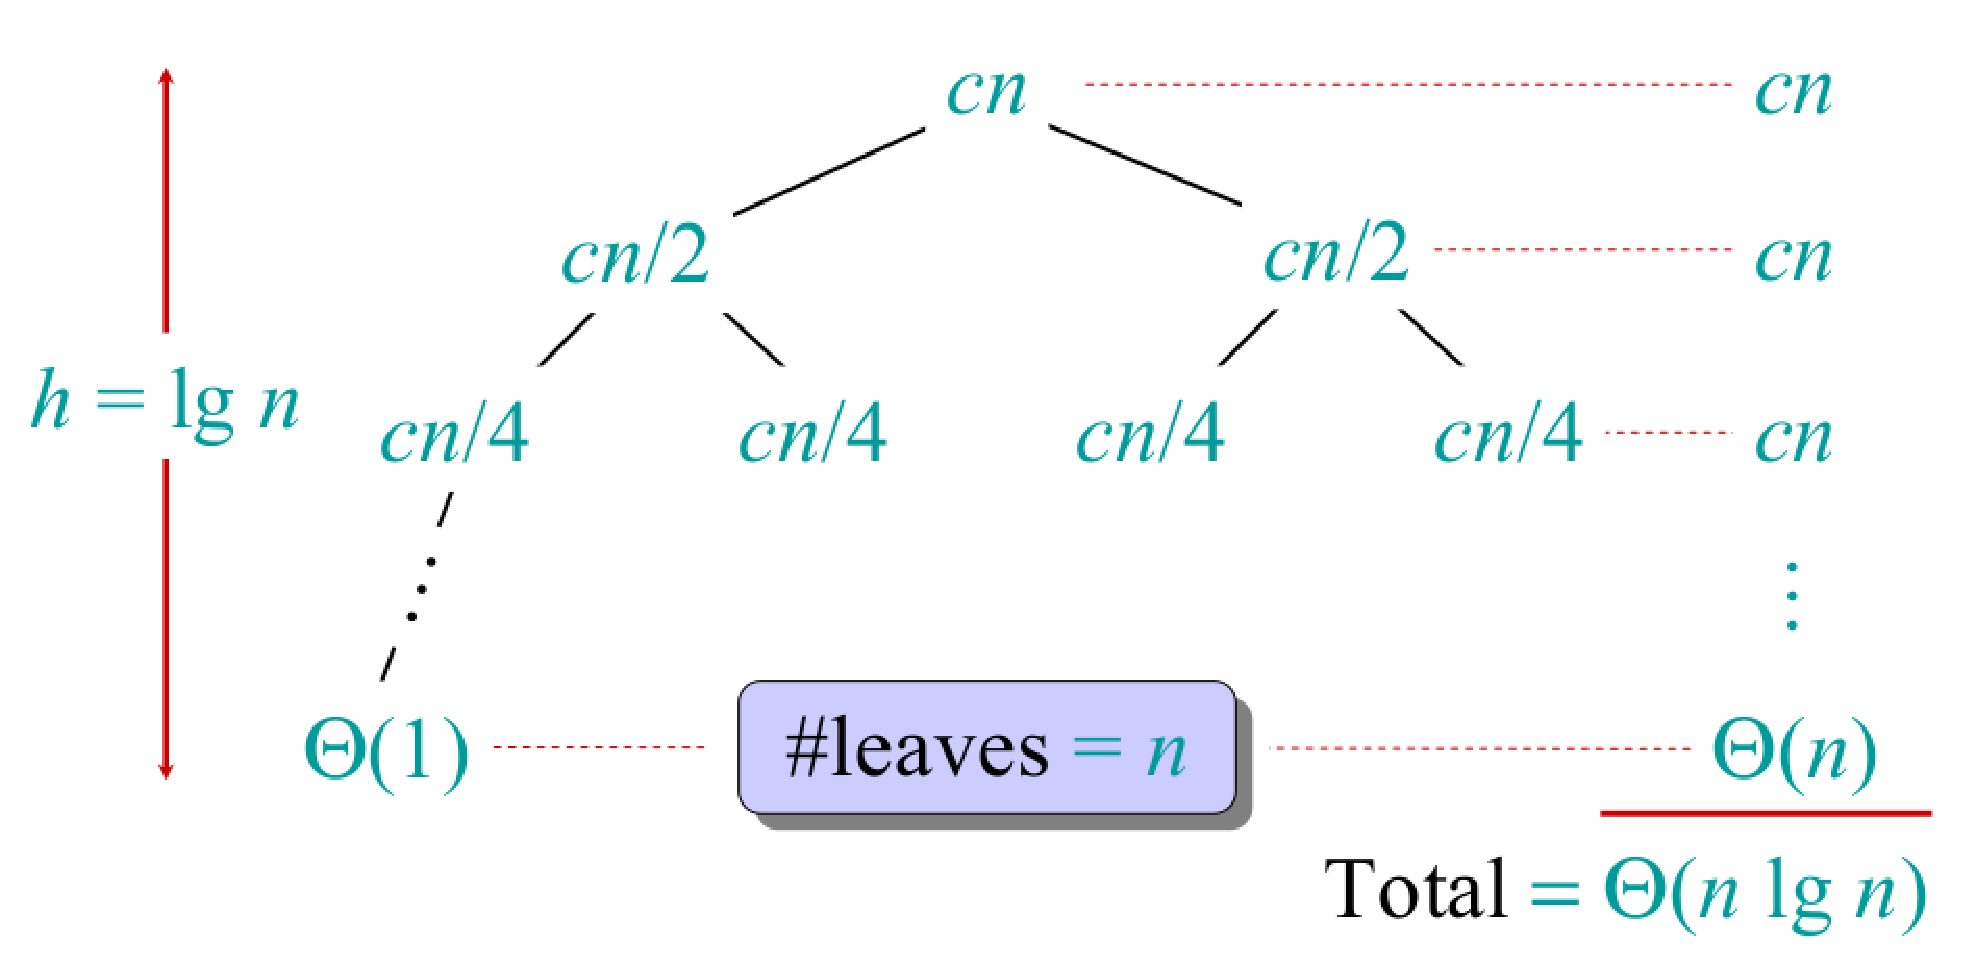
\includegraphics[width=4in]{lecture1/tree10.eps}
  \caption{Дерево рекурсии}
  \label{fig:rectree10}
\end{figure}

Выводы: поскольку $\Theta(n lgn)$ растёт намного медленнее, чем $\Theta(n^2)$, то
сортировка слиянием использует намного меньше операций и потому работает
быстрее. Это становится заметно на практике уже при $n > 30$

\end{document}
